\newprob{1719220648}
{
    % active phys p283 q2
    在一個穩定而勻強的垂直向上磁場內,一個金圈 環水平擺放,如圖。在以下哪一個情況中,環上 會感生電流?
    \par{\par\centering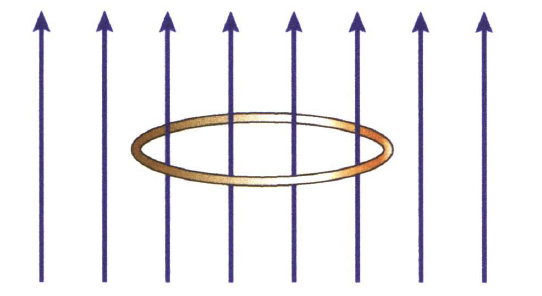
\includegraphics[width=.3\textwidth]{./img/ch5_induction_mc_2024-06-24-17-18-21.png}\par}
    \begin{tasks}
        \task 金屬環以恆速水平移動。
        \task 金屬環以勻加速度水平移動。
        \task 金屬環繞直徑勻速轉動。
        \task 以上皆會。
    \end{tasks}
}{C}

\newprob{1719220710}
{
    % active phys p283 q3
    當一條導線在一塊磁鐵旁移動時,其上\textbf{必定}感生 以下哪一項?
    \begin{tasks}
        \task 電流
        \task 電壓
        \task 兩者皆會
        \task 兩者皆非
    \end{tasks}
}{B}

\newprob{1719220769}
{
    % active phys p283 q4
    一根金屬棒在一個匀強磁場中以初速$v_0$向上拋 出,移動時切割磁場線。金屬棒能達到的最大高 度為多少?忽略空氣阻力。
    \begin{tasks}
        \task 低於$\dfrac{v^2_0}{2g}$
        \task 等於$\dfrac{v^2_0}{2g}$
        \task 高於$\dfrac{v^2_0}{2g}$
        \task 視乎磁場方向
    \end{tasks}
}{B}

\newprob{1719219575}
{
    % active phys p311 q2
    以下哪一項不是磁通量的單位?
    \begin{tasks}
        \task \unit{Wb}
        \task \unit{V.s^{-1}}
        \task \unit{T.m^2}
        \task \unit{N.m.A^{-1}}
    \end{tasks}
}{B}

\newprob{1719219972}
{
    % active phys p311 q4
    一個扁平線圈由一條10 cm 長的銅線繞成,在圖 中沿 y 方向的匀強磁場內繞z軸旋轉。
    \par{\par\centering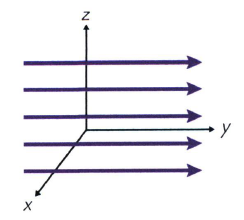
\includegraphics[width=.3\textwidth]{./img/ch5_induction_mc_2024-06-24-17-06-53.png}\par}
    為得到最大的感生電流,線圈應繞成哪一種形 狀?所處的平面應為哪一個?
    \begin{tasks}
        \task [] 形狀 \tab\tab 處於
        \task 方形 \tab\tab xy 平面
        \task 方形 \tab\tab xz 平面
        \task 圓形 \tab\tab xy 平面
        \task 圓形 \tab\tab xz 平面
    \end{tasks}
}{D}

\newprob{1719216701}
{
    % active phys p334 q2
    一個輕巧而有彈性的導電環自由地掛在一條平滑 路軌上,並同時位於一個同軸的螺線管中央。螺 線管以串聯方式連接至一個變阻器和一個電池組。
    \par{\par\centering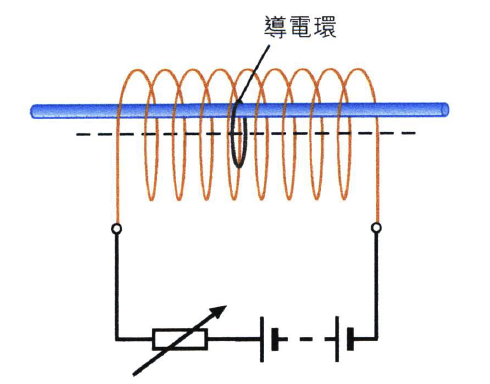
\includegraphics[width=.3\textwidth]{./img/ch5_induction_mc_2024-06-24-16-49-17.png}\par}
    若變阻器的電阻增加,導電環發生甚麼事情?
    \begin{tasks}
        \task 向左移。
        \task 向右移。
        \task 面積增加。
        \task 面積減少。
    \end{tasks}
}{C}

\newprob{1719218989}
{
    % active phys p334 q3
    一對平行的長直導線載有相同的電流1。一個長方 形線圈從位置X 以恆速移至位置Y,如圖。
    \par{\par\centering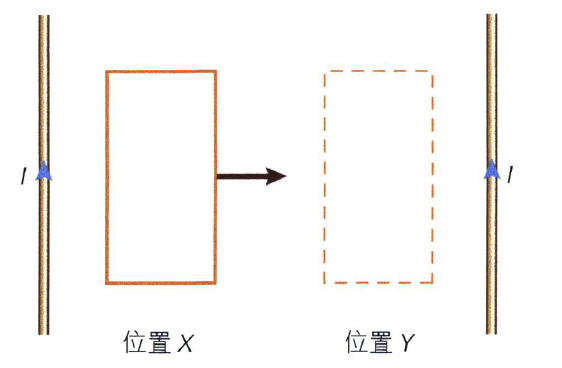
\includegraphics[width=.35\textwidth]{./img/ch5_induction_mc_2024-06-24-16-53-10.png}\par}
    以下哪一項正確描述線圈上感生的電流方向?
    \begin{tasks}
        \task 整個過程為順時針
        \task 𤨣個過程為逆時針
        \task 先順時針,後逆時針
        \task 先逆時針,後順時針
    \end{tasks}
}{A}

\newprob{1719219197}
{
    % active phys p334 q4
    一塊蹄形磁鐵懸在一塊銅碟上方,如圖。圓碟可 繞通過中心的垂直軸自由旋轉。
    \par{\par\centering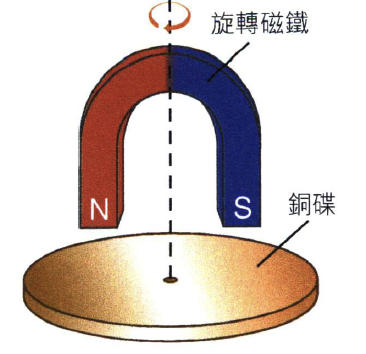
\includegraphics[width=.25\textwidth]{./img/ch5_induction_mc_2024-06-24-16-54-03.png}\par}
    從上方觀察,若磁鐵沿順時針方向旋轉,銅碟會 發生甚麼事情?
    \begin{statements}
        \task 從上方觀察,銅碟沿逆時針方向旋轉。
        \task 磁力作用在蹄形磁鐵上,並抗衡其運動。
        \task 銅碟會逐漸變熱。
    \end{statements}
    \begin{tasks}
        \task 只有(1)和(2)
        \task 只有(1)和(3)
        \task 只有(2)和(3)
        \task (1), (2) 和 (3)
    \end{tasks}
}{C}

\newprob{1719219274}
{
    % active phys p334 q5
    一個探察線圈連接至一個檢流計,然後放在一個 匀強磁場中,如圖。線圈的平面與磁場互相垂直。
    \par{\par\centering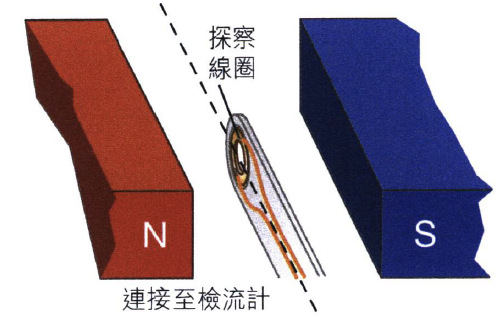
\includegraphics[width=.3\textwidth]{./img/ch5_induction_mc_2024-06-24-16-54-54.png}\par}
    怎樣能令檢流計指針偏轉?
    \begin{statements}
        \task 沿磁場線方向前後移動線圈。
        \task 把線圈抽離磁場。
        \task 沿虛線旋轉線圈。
    \end{statements}
    \begin{tasks}
        \task 只有(1)
        \task 只有(3)
        \task 只有(1)和(2)
        \task 只有(2)和(3)
    \end{tasks}
}{D}

\newprob{1719219333}
{
    % active physics q6
    一個長直螺線管繞在一個紙筒上,橫截面積為  \qty{6.0}{cm^2} ,線圈密度為每米1500匝,並載有1 A的 電流。另有一個15匝的線圈,橫截面積為  \qty{30}{cm^2} , 如圖示般圍着長直螺線管。
    \par{\par\centering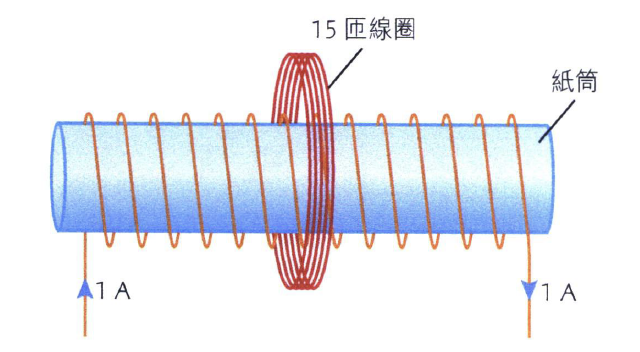
\includegraphics[width=.35\textwidth]{./img/ch5_induction_mc_2024-06-24-16-56-43.png}\par}
    假如長直螺線管中的電流在0.01 s內穩定減少至 零,線圈中的感生電動勢為多少?
    \begin{tasks}
        \task 0.113 mV
        \task 1.70 mV
        \task 3.38 mV
        \task 8.46 mV
    \end{tasks}
}{B}

\newprob{1719219490}
{
    % HKDSE 練習卷
    一個邊長為L的正方形金屬框放 置於一個勻強磁場B之中,如圖所示。當金屬框 沿XY 軸分別旋轉 \dg{90} 和 \dg{180} 時,通過金屬框磁 通量的改變是多少?
    \par{\par\centering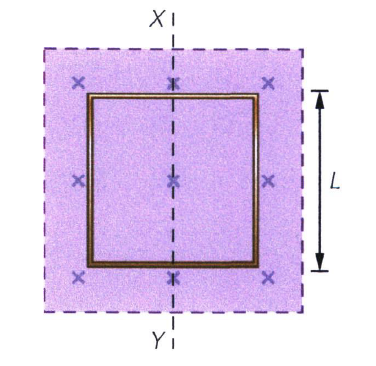
\includegraphics[width=.25\textwidth]{./img/ch5_induction_mc_2024-06-24-16-58-27.png}\par}
    \begin{tasks}
        \task [] \dg{90} \tab\tab \dg{180}
        \task $0$ \tab\tab $0$
        \task $0$ \tab\tab $2BL^2$
        \task $BL^2$ \tab\tab $0$
        \task $BL^2$ \tab\tab $2BL^2$
    \end{tasks}
}{D}

